\documentclass{ctexart}
\usepackage{graphicx}
\usepackage{caption}
\usepackage{float}
\usepackage{amsmath}
\usepackage{fancyhdr}
\usepackage{xunicode-addon}
\usepackage{booktabs}
\usepackage{listings}
\usepackage{hyperref}
\usepackage[a4paper,hmargin=1.25in,vmargin=1in]{geometry}
% !TeX program = xelatex
\lstdefinestyle{mystyle}{
  basicstyle=\ttfamily\footnotesize,
  breakatwhitespace=false,         
  breaklines=true,                 
  captionpos=b,                    
  keepspaces=true,                 
  numbers=left,                    
  numbersep=5pt,                  
  showspaces=false,                
  showstringspaces=false,
  showtabs=false,                  
  tabsize=2
}

\lstset{style=mystyle}

\title{\begin{figure}[H]
	\centering 
	\includegraphics[height=7cm,width=14cm]{E:/Pictures/中科大.jpg}
	\end{figure}\Huge\textbf{数据结构实验报告4}\\\huge{图及相关应用}}
\date{}
\punctstyle{banjiao} 
\pagestyle{fancy}
	\fancyhead[C]{\LARGE\textbf{实验报告4}}
	\fancyhead[L]{}
	\fancyhead[R]{}
	\fancyfoot[C]{\thepage}
\begin{document}
	\maketitle
	\thispagestyle{empty}
	
	\[\makebox{\Large{姓名:\underline{\makebox[5cm]{高茂航}}}}\]
	
    \[\makebox{\Large{学号:\underline{\makebox[5cm]{PB22061161}}}}\]
	
	\[\makebox{\Large{日期:\underline{\makebox[5cm]{2023年11月30日}}}}\]
	
	\clearpage

	\pagenumbering{arabic}

	\section{图的遍历}
输入一个无向图,输出图的深度优先搜索遍历顺序与广度优先搜索遍历顺序。当有多个节点可以搜索时,
优先去节点编号最小的那个。
	
	\subsection{算法描述}
	\subsubsection{数据结构}
	\begin{lstlisting}[language=C++, caption=数据结构]
		typedef int VertexType;
		#define MaxVexNum 30
		#define INFINITY 65535
		typedef struct{
			VertexType ves[MaxVexNum+1];//顶点表
			int arc[MaxVexNum+1][MaxVexNum+1];//邻接矩阵
			int VertexNum,EdgeNum;//分别是图中当前顶点数和边数
		}MGraph;
		int visited[MaxVexNum+1]={0};//记录每个顶点是否被访问过,0为未访问,1为已访问
		typedef struct QueueList{
			int vertex;//存顶点序号
			struct QueueList* next;
		}Queue;
	\end{lstlisting}
	\subsubsection{程序结构}
	\begin{lstlisting}[language=C++, caption=程序结构]
		void CreateMGraph(MGraph &);//创建无向图的邻接矩阵结构
		void DFS(MGraph &,int);//深度优先算法(邻接矩阵)
		void DFSTraverse(MGraph &,int);//深度优先遍历操作(邻接矩阵)
		void BFSTraverse(MGraph &,int);//广度优先遍历操作(邻接矩阵)
		void EnQueue(Queue** Q,int n);//把序号为n的顶点入队
		int DeQueue(Queue** Q);//将队首顶点出队,返回其序号
		int QueueEmpty(Queue *Q);//判断队列是否为空
		int main(){
			MGraph G;
			int a,i;
			CreateMGraph(G);
			cin>>a;//输入遍历起始的起始顶点
			DFSTraverse(G,a);
			for(i=0;i<=G.VertexNum;i++)
				visited[i]=0;
			BFSTraverse(G,a);
		}
	\end{lstlisting}
	\subsubsection{主要算法}
	\begin{lstlisting}[language=C++, caption=创建无向图的邻接矩阵结构]
		void CreateMGraph(MGraph &G){//创建无向图的邻接矩阵结构
		int i=0,j=0,k=0;
		cin>>G.VertexNum>>G.EdgeNum;
		for(i=1;i<=G.VertexNum;i++)
			G.ves[i]=i;//顶点序号从1开始
		for(i=1;i<=G.VertexNum;i++)
			for(j=1;j<=G.VertexNum;j++){
				if(i==j)
					G.arc[i][j]=0;
				else
					G.arc[i][j]=INFINITY;
			}
		for(k=1;k<=G.EdgeNum;k++){
			cin>>i>>j;
			G.arc[j][i]=G.arc[i][j]=1;   
		}
	}
	\end{lstlisting}
	\begin{lstlisting}[language=C++, caption=深度优先搜索算法]
		void DFS(MGraph &G,int a){//深度优先算法(邻接矩阵)
		int i=0;
		visited[a]=1;
		cout<<G.ves[a];
		for(i=1;i<=G.VertexNum;i++)
			if(G.arc[a][i]==1&&!visited[i])
				DFS(G,i);
	}
	void DFSTraverse(MGraph &G,int a){//深度优先遍历操作(邻接矩阵)
		int i=0;
		for(i=1;i<=G.VertexNum;i++)
			visited[i]=0;
		DFS(G,a);
	}
	\end{lstlisting}
	\begin{lstlisting}[language=C++, caption=广度优先搜索算法]
		void BFSTraverse(MGraph &G,int a){//广度优先遍历操作(邻接矩阵)
		int i=0,j=0,ver=0;
		for(i=1;i<=G.VertexNum;i++)
			visited[i]=0;
		Queue* Q=NULL;
		visited[a]=1;
		cout<<G.ves[a];
		EnQueue(&Q,a);
		while(!QueueEmpty(Q)){
			i=DeQueue(&Q);
			for(j=1;j<=G.VertexNum;j++){
				if(G.arc[i][j]==1&&!visited[j]){
					visited[j]=1;
					cout<<G.ves[j];
					EnQueue(&Q,j);
				}
			}
		}	
	}	
	\end{lstlisting}
	\subsection{测试结果}
	\begin{figure}[H]
		\centering 
		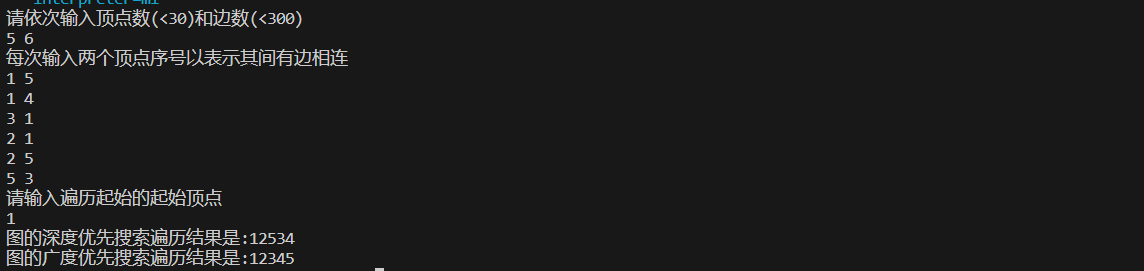
\includegraphics[height=3cm,width=12cm]{1.png}
		\end{figure}
\section{求最小生成树}
输入一个无向图,用 Prim 和 Kruskal 算法计算最小生成树并输出。

\subsection{算法描述}

\subsubsection{数据结构}
\begin{lstlisting}[language=C++, caption=数据结构(Prim)]
	typedef int VertexType;
typedef struct{
    VertexType ves[MaxVexNum+1];//顶点表
    int arc[MaxVexNum+1][MaxVexNum+1];//邻接矩阵
    int VertexNum,EdgeNum;//分别是图中当前顶点数和边数
}MGraph;
\end{lstlisting}
\begin{lstlisting}[language=C++, caption=数据结构(Kruskal)]
	typedef int VertexType;
typedef struct{
    VertexType ves[MaxVexNum+1];//顶点表
    int arc[MaxVexNum+1][MaxVexNum+1];//邻接矩阵
    int VertexNum,EdgeNum;//分别是图中当前顶点数和边数
}MGraph;
typedef struct{
	int begin;
	int end;
	int weight;
}Edge;//边集数组结构
Edge edges[MaxEdgeNum+1];//边集数组	
\end{lstlisting}
\subsubsection{程序结构}
\begin{lstlisting}[language=C++, caption=程序结构(Prim)]
	void CreateMGraph(MGraph &);//创建无向图的邻接矩阵结构
	void Prim(MGraph);//Prim算法求最小生成树的各边的长度之和
	int main(){
		MGraph G;
		CreateMGraph(G);
		Prim(G);
	}
\end{lstlisting}
\begin{lstlisting}[language=C++, caption=程序结构(Kruskal)]
	void CreateMGraph(MGraph &);//创建无向图的邻接矩阵结构
	void Kruskal(MGraph);//Kruskal算法求最小生成树的各边的长度之和
	void SortEdge(Edge *);//将边集数组按权值从小到大排序
	int Find(int* parent,int i);//查找连线顶点的尾部下标
	int main(){
		MGraph G;
		CreateMGraph(G);
		Kruskal(G);
	}
\end{lstlisting}
\subsubsection{主要算法}
	\begin{lstlisting}[language=C++, caption=Prim算法求最小生成树的各边的长度之和]
		void Prim(MGraph G){//Prim算法求最小生成树的各边的长度之和
		int min=0,length=0,i=0,j=0,k=0;
		int adjvex[MaxVexNum+1]={0};//记录已加入生成树的顶点序号,adjvex[i]的值是生成树上i顶点上一个连接的顶点序号
		int lowcost[MaxVexNum+1]={0};//记录已遍历顶点的邻边中最小的权重
		lowcost[1]=0;
		adjvex[1]=1;
		for(i=2;i<=G.VertexNum;i++){
			lowcost[i]=G.arc[1][i];
			adjvex[i]=1;
		}
		for(i=1;i<G.VertexNum;i++){
			min=INFINITY;
			j=2;
			k=1;
			while(j<=G.VertexNum){
				if(lowcost[j]&&lowcost[j]<min){
					min=lowcost[j];
					k=j;
				}
				j++;
			}
			length+=G.arc[k][adjvex[k]];
			lowcost[k]=0;//此顶点已完成任务
			for(j=2;j<=G.VertexNum;j++){
				if(lowcost[j]&&G.arc[k][j]<lowcost[j]){
					lowcost[j]=G.arc[k][j];
					adjvex[j]=k;
				}
			}
		}
		cout<<"最小生成树的各边的长度之和为"<<length;
	}
	\end{lstlisting}
	\begin{lstlisting}[language=C++, caption=创建并排序编辑数组(Kruskal)]
		void CreateMGraph(MGraph &G){//创建无向图的邻接矩阵结构和边集数组
		int i=0,j=0,k=0,w;
		cout<<"请依次输入顶点数(<30)和边数(<300)"<<endl;
		cin>>G.VertexNum>>G.EdgeNum;
		for(i=1;i<=G.VertexNum;i++)
			G.ves[i]=i;//顶点序号从1开始
		for(i=1;i<=G.VertexNum;i++)
			for(j=1;j<=G.VertexNum;j++){
				if(i==j)
					G.arc[i][j]=0;
				else
					G.arc[i][j]=INFINITY;
			}
		for(k=1;k<=G.EdgeNum;k++){//输入边的信息
			cin>>i>>j>>w;
			G.arc[j][i]=G.arc[i][j]=w;
			edges[k].begin=i;
			edges[k].end=j;
			edges[k].weight=w;
		}
		for(k=G.EdgeNum+1;k<=MaxEdgeNum;k++)
			edges[k].weight=0;
		for(k=1;k<=G.EdgeNum;k++)
			cout<<edges[k].begin<<" "<<edges[k].end<<" "<<edges[k].weight<<endl;
		cout<<endl;
		SortEdge(edges);//将边集数组按权值从小到大排序
		for(k=1;k<=G.EdgeNum;k++)
			cout<<edges[k].begin<<" "<<edges[k].end<<" "<<edges[k].weight<<endl;
	}
	void SortEdge(Edge *edges){//将边集数组按权值从小到大排序
		int i,j,temp;
		for(i=1;i<=MaxEdgeNum;i++){
			for(j=1;j<=MaxEdgeNum;j++){
				if(edges[j].weight>edges[j+1].weight&&edges[j+1].weight){
					temp=edges[j].begin;
					edges[j].begin=edges[j+1].begin;
					edges[j+1].begin=temp;
					temp=edges[j].end;
					edges[j].end=edges[j+1].end;
					edges[j+1].end=temp;
					temp=edges[j].weight;
					edges[j].weight=edges[j+1].weight;
					edges[j+1].weight=temp;
				}
			}
		}
	}
	\end{lstlisting}
	\begin{lstlisting}[language=C++, caption=Kruskal算法求最小生成树的各边的长度之和]
		void Kruskal(MGraph G){//Kruskal算法求最小生成树的各边的长度之和
		int i,n,m,length=0;
		int parent[MaxVexNum+1];//定义一数组用来判断边与边是否形成环路,parent[m]=n表示m与n在同一集合中,而不是表示m和n之间有边
		for(i=0;i<=G.VertexNum;i++)
			parent[i]=0;
		for(i=1;i<=G.EdgeNum;i++){
			n=Find(parent,edges[i].begin);
			m=Find(parent,edges[i].end);
			if(n!=m){//如果n与m不等,说明此边没有与现有生成树形成环路
				parent[n]=m;//将此边的结尾顶点放入下标为起点的parent中,表示此顶点已经在生成树集合中
				length+=edges[i].weight;
			}
		}
		cout<<"最小生成树的各边的长度之和为"<<length;
	}
	\end{lstlisting}
	\subsection{测试结果}
	\begin{figure}[H]
		\centering 
		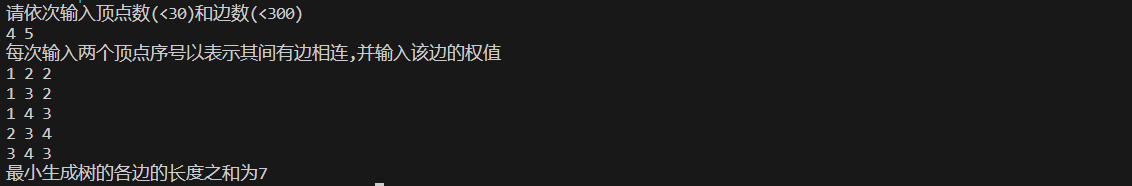
\includegraphics[height=2cm,width=12cm]{2.png}
		\end{figure}
	\section{求最短路径}
	输入一个无向铁路交通图、始发站和终点站,用 Dijkstra 算法计算从始发
站到终点站的最短路径。
	\subsection{算法描述}
	\subsubsection{数据结构}
	\begin{lstlisting}[language=C++, caption=数据结构]
		typedef struct{
			VertexType ves[MaxVexNum+1];//顶点表
			int arc[MaxVexNum+1][MaxVexNum+1];//邻接矩阵
			int VertexNum,EdgeNum;//分别是图中当前顶点数和边数
		}MGraph;
	\end{lstlisting}
	

	\subsubsection{程序结构}
	\begin{lstlisting}[language=C++, caption=程序结构]
		int Patharc[MaxVexNum];//Patharc[v]的值为最短路径下前驱顶点的坐标
		int ShortestPath[MaxEdgeNum];//储存起点到各点最短路径的权值和
		void CreateMGraph(MGraph &);//创建无向图的邻接矩阵结构
		void Dijkstra(MGraph, int start,int end);//Dijkstra算法求最短路径
		int main(){
			int start,end;
			MGraph G;
			CreateMGraph(G);
			cin>>start>>end;
			Dijkstra(G,start,end);
		}
	\end{lstlisting}
	\subsubsection{主要算法}
	\begin{lstlisting}[language=C++, caption=Dijkstra算法求求start到end最短路径]
		void Dijkstra(MGraph G, int start,int end){//Dijkstra算法求求start到end最短路径
		int i,j,k,min;
		int Final[MaxVexNum];//Final[v]为1表示已经求得从start到v的最短路径
		for(i=1;i<=G.VertexNum;i++){//初始化
			Final[i]=0;
			ShortestPath[i]=G.arc[start][i];
			Patharc[i]=-1;
		}
		ShortestPath[start]=0;//start到start的最短路径为0
		Final[start]=1;//start到start的最短路径已经求得
		for(i=1;i<G.VertexNum;i++){//每次循环求得从start到某个顶点v的最短路径
			min=INFINITY;
			for(j=1;j<=G.VertexNum;j++){//找到当前未求得最短路径的顶点中距离start最近的顶点
				if(!Final[j]&&ShortestPath[j]<min){
					k=j;
					min=ShortestPath[j];
				}
			}
			Final[k]=1;
			for(j=1;j<=G.VertexNum;j++){//修正当前最短路径及距离
				if(!Final[j]&&min+G.arc[k][j]<ShortestPath[j]){
					ShortestPath[j]=min+G.arc[k][j];
					Patharc[j]=k;
				}
			}
		}
		cout<<"从"<<start<<"到"<<end<<"的最短路径是"<<ShortestPath[end];
	}	
	\end{lstlisting}
	\subsection{测试结果}
	\begin{figure}[H]
		\centering 
		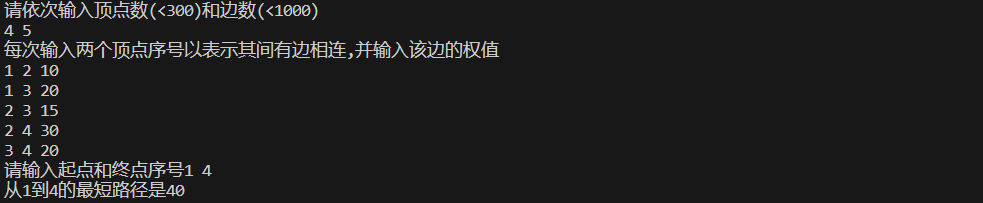
\includegraphics[height=2.5cm,width=12cm]{3.png}
		\end{figure}
	\section{调试分析}
本实验主要是图的一些基本操作,问题主要出现在处理各个数组的过程中,需要理清它们之间的关系以及它们的作用,否则很容易出错。
	\section{算法时空分析}
	由于本实验的图都采用邻接矩阵的方式存储,所以空间复杂度都是$O(n^2)$,
DFS和BFS的时间复杂度都是$O(n^2)$,Prim算法的时间复杂度是$O(n^2)$,Kruskal算法的时间复杂度是$O(nlogn)$,Dijkstra算法的时间复杂度是$O(n^2)$。
	
	\section{实验体会收获}
通过本实验,我加深了对图的一些基本算法的理解,对图的遍历、求最小生成树和最短路径的操作更加熟悉,为将来进一步学习算法基础做了准备。
	
\end{document}